\documentclass[10pt,a4paper]{article}
\usepackage[utf8]{inputenc}
\usepackage[T1]{fontenc}
\usepackage[spanish,es-noquoting]{babel}
\usepackage[margin=1.8cm]{geometry}
\usepackage{amsmath,amssymb,mathtools}
\usepackage{graphicx}
\usepackage{subcaption}
\usepackage{booktabs}
\usepackage{hyperref}
\usepackage{xcolor}
\usepackage[section]{placeins}
\graphicspath{{../figures/}}
\setlength{\parskip}{0.4em}
\setlength{\parindent}{0pt}
\setlength{\emergencystretch}{3em}
\newcommand{\real}[1]{\textcolor{red}{#1}}

\title{\vspace{-1.5cm}TP2 -- Reconstrucción 3D por estéreo multivista\\[0.2em]
\large I308 Visión Artificial -- Universidad de San Andrés}
\author{Franco Needleman \and Lautaro García Conejero \and Luca Fassio}
\date{Octubre 2026}

\begin{document}
\maketitle
\vspace{-0.8cm}

\begin{abstract}
Reconstruimos la nube de puntos 3D métrica de un caracol marino a partir de 83 pares
estéreo tomados en órbita con una cámara ELP-USB3D1080P02-H120, usando un tablero ChArUco
como marco de referencia global. El pipeline calibra y rectifica el par estéreo, calcula
disparidad con SGBM, estima la pose de cada toma con \texttt{solvePnP}, fusiona las nubes en el
marco del tablero y las optimiza con Open3D. Estimamos un tamaño de
$122\times219\times202$\,mm (alto $\times$ largo $\times$ ancho)\real{, frente a \dots\ medidos con regla}.
\end{abstract}

%=====================================================================
\section{Introducción y marco teórico}

\textbf{Modelo pinhole y distorsión.} Un punto $\mathbf{X}_c=(X,Y,Z)$ en coordenadas de cámara
se proyecta en $u = f_x X/Z + c_x$, $v = f_y Y/Z + c_y$, o en forma matricial
$\lambda\,\tilde{\mathbf{u}} = K[R\,|\,\mathbf{t}]\tilde{\mathbf{X}}$ con
$K=\begin{psmallmatrix} f_x & 0 & c_x\\ 0 & f_y & c_y \\ 0&0&1\end{psmallmatrix}$.
Los \emph{parámetros intrínsecos} son las distancias focales en píxeles $(f_x,f_y)$ y el punto
principal $(c_x,c_y)$. Las lentes reales agregan distorsión radial ($k_1,k_2,k_3$) y tangencial
($p_1,p_2$), que curvan las rectas. Hay que calibrar porque estos parámetros dependen de cada
cámara y sin ellos no se puede relacionar un píxel con un rayo 3D, ni medir en milímetros.

\textbf{Calibración estéreo.} Además de los intrínsecos de cada cámara, se estiman los
\emph{extrínsecos relativos} $(R,\mathbf{t})$ que llevan puntos del sistema de la cámara izquierda
al de la derecha: $\mathbf{X}_r = R\mathbf{X}_l+\mathbf{t}$. La norma $\|\mathbf{t}\|$ es la
\emph{baseline} y fija la escala métrica de la triangulación. Se estiman observando un patrón
de geometría conocida (checkerboard) en muchas poses: para cada imagen se detectan las esquinas,
y se minimiza por Levenberg--Marquardt la suma de los cuadrados de las distancias entre las
esquinas detectadas y las proyectadas por el modelo, de forma conjunta sobre $K_l, K_r$,
distorsiones, $(R,\mathbf{t})$ y la pose del patrón en cada vista (\texttt{cv.stereoCalibrate}).
El \emph{error de reproyección} RMS es la raíz del promedio de esas distancias en píxeles y
mide qué tan bien explica el modelo las observaciones.

\textbf{Geometría epipolar y rectificación.} Dado un punto en la imagen izquierda, su
correspondiente en la derecha está sobre una recta, la \emph{línea epipolar}
($\tilde{\mathbf{u}}_r^\top F\tilde{\mathbf{u}}_l=0$). La rectificación aplica a cada imagen una
homografía (rotaciones $R_1, R_2$ y nuevas proyecciones $P_1,P_2$, \texttt{cv.stereoRectify}) y
quita la distorsión, de modo que ambos planos imagen quedan coplanares y las líneas epipolares
son horizontales y en la misma fila. Así la búsqueda de correspondencias pasa de 2D a 1D:
para cada píxel solo se busca a lo largo de la misma fila, lo que hace viable y robusto el
cálculo denso de disparidad.

\textbf{De disparidad a profundidad.} En un par rectificado, con focal $f$ y baseline $B$, un
punto a profundidad $Z$ aparece en columnas $x_l$ y $x_r$ con disparidad $d=x_l-x_r$ y, por
triángulos semejantes, $Z = fB/d$. La profundidad es inversamente proporcional a la
disparidad, así que el error crece como $\delta Z \approx Z^2\,\delta d/(fB)$. La matriz $Q$ de
\texttt{stereoRectify} expresa esta relación en forma homogénea:
$[X\,Y\,Z\,W]^\top = Q[x\;y\;d\;1]^\top$ (\texttt{cv.reprojectImageTo3D}).

%=====================================================================
\section{Metodología}

\textbf{Dataset propio.} Usamos la cámara ELP de la cátedra (dos sensores de $1920\times1080$,
baseline nominal de 60\,mm). Tomamos 52 pares de calibración con un checkerboard de
$9\times6$ esquinas internas y cuadros de 28\,mm, y 83 pares del objeto en una órbita completa
sobre un ChArUco de $9\times13$ cuadros de 42\,mm (marcadores de 31.5\,mm, \texttt{DICT\_5X5\_100}),
que es el marco global ($x,y$ sobre el tablero, $z$ hacia la mesa).

\textbf{Calibración.} Implementada con funciones de OpenCV (\texttt{src/calibration.py}).
Las esquinas se detectan con \texttt{findChessboardCorners} sobre la imagen reducida al 70\,\% y
se refinan con \texttt{cornerSubPix} a resolución completa. Se calibra con
\texttt{stereoCalibrateExtended}, que devuelve el error por vista, y se descartan
iterativamente los pares con error atípico (umbral: mediana $+\,2.5\cdot1.4826\cdot$MAD, con piso de
1\,px); se usaron 32 pares. Como la órbita de captura cubre distancias y ángulos distintos a
los de la calibración, refinamos $(R,\mathbf{t})$ con 12 vistas del ChArUco (capturas 0, 6, \dots,
66) fijando los intrínsecos (\texttt{CALIB\_FIX\_INTRINSIC}). Validamos este paso en los 71 pares
restantes. Los mapas de rectificación se calculan con \texttt{stereoRectify} ($\alpha=0$) e
\texttt{initUndistortRectifyMap}.

\textbf{Disparidad.} \texttt{StereoSGBM} (\texttt{src/disparity.py}) sobre las imágenes rectificadas
en grises: \texttt{numDisparities}=192 (cubre de $\sim$190\,mm al infinito, ya que
$Z=fB/d\approx 600\cdot59/192$), \texttt{blockSize}=7, $P_1=8\cdot7^2$, $P_2=32\cdot7^2$ (suavidad
estándar de OpenCV), \texttt{uniquenessRatio}=5, \texttt{speckleWindowSize}=100,
\texttt{speckleRange}=2, \texttt{disp12MaxDiff}=1 (chequeo izquierda-derecha). Los valores se
ajustaron visualmente: bloques más chicos generaban ruido en el tablero blanco, y una
unicidad mayor vaciaba las zonas de poca textura.

\textbf{Nube local y pose global.} La nube local se obtiene con \texttt{reprojectImageTo3D}
y $Q$, conservando los píxeles con $d>0$ y $Z>0$, y el color de la imagen izquierda. Está
expresada en la cámara izquierda \emph{rectificada}. La pose se estima detectando el ChArUco
en la imagen izquierda \emph{original} (\texttt{CharucoDetector}) y resolviendo
\texttt{solvePnP} con $K_l$ y la distorsión izquierda. Se rechazan las tomas con menos de 8
esquinas, esquinas colineales, cobertura menor al 2\,\% de la imagen o RMS de reproyección
mayor a 5\,px. \texttt{solvePnP} devuelve $(\mathbf{r},\mathbf{t})$ tales que
$\mathbf{X}_c = R\,\mathbf{X}_w+\mathbf{t}$, donde $\mathbf{r}$ es el \emph{vector de Rodrigues}: su
dirección es el eje de giro y su norma el ángulo en radianes. \texttt{cv.Rodrigues} lo
convierte en la matriz $R$. La transformación de la nube al mundo es
\[
\mathbf{X}_w \;=\; \underbrace{\begin{bmatrix}R^\top & -R^\top\mathbf{t}\\ \mathbf{0}^\top&1\end{bmatrix}}_{T_{w\leftarrow c}}
\underbrace{\begin{bmatrix}R_1^\top & \mathbf{0}\\ \mathbf{0}^\top&1\end{bmatrix}}_{T_{c\leftarrow \text{rect}}}\;\mathbf{X}_{\text{rect}},
\]
donde $R_1^\top$ deshace la rotación de rectificación y $T_{w\leftarrow c}$ invierte la pose de PnP.

\textbf{Fusión y optimización} (\texttt{src/fusion.py}). Las capturas se procesan de a una, sin
acumular nunca las nubes completas ($\sim$1.4\,M puntos cada una):
\begin{enumerate}\setlength{\itemsep}{0pt}
\item \emph{Corrección por plano del tablero.} La profundidad estéreo y la pose PnP difieren
unos milímetros por vista, así que el tablero reconstruido no cae exactamente en $z=0$.
Se ajusta un plano con RANSAC (\texttt{segment\_plane}, umbral de 2\,mm) a los puntos cercanos al
tablero, y se aplica la rotación y traslación mínimas que lo llevan a $z=0$.
\item \emph{Filtrado espacial}: se seleccionan los puntos dentro de una
\texttt{OrientedBoundingBox} alineada al tablero (\texttt{get\_point\_indices\_}\allowbreak\texttt{within\_bounding\_box}
y \texttt{select\_by\_index}), con $x\in[40,290]$, $y\in[140,410]$ y $z\in[-160,-2]$\,mm. El límite
$z<-2$\,mm excluye la superficie del tablero.
\item \emph{ICP punto a plano} (opcional) de cada captura contra una primera fusión limpia
(distancia máxima de 3\,mm).
\item \emph{Consistencia multivista}: se conservan los voxels de 3\,mm observados por al menos 20
capturas. Los \emph{flying pixels} que SGBM genera en los bordes de profundidad (interpolando
entre el objeto y el tablero) y los fragmentos flotantes dependen del punto de vista, por lo que
pocas capturas los respaldan. La superficie real aparece en decenas.
\item \emph{Submuestreo} con \texttt{voxel\_down\_sample} de 1\,mm: conserva el detalle de las
espinas del caracol y reduce la redundancia entre vistas.
\item \emph{Outliers}: \texttt{remove\_statistical\_outlier} (30 vecinos, $2\sigma$) y luego el
cluster DBSCAN más grande ($\varepsilon=5$\,mm).
\end{enumerate}
Por último se estiman normales (radio de 4\,mm, orientadas hacia afuera), se exporta
\texttt{caracol.ply} en binario y se genera una malla de Poisson (profundidad 9) como opcional.

\textbf{Medición métrica.} El alto es la distancia al plano $z=0$ del punto más alto (percentil
99.5 de $-z$). El largo y el ancho son los lados del rectángulo de área mínima
(\texttt{cv.minAreaRect}) que encierra la proyección de la nube sobre el tablero, lo que equivale a
una \emph{bounding box} orientada con un eje vertical. El resultado es métrico, y no ``salvo
escala'' como en la estructura a partir del movimiento monocular, por dos razones: la baseline
$B$ se calibró con un patrón de tamaño conocido, lo que fija $Z=fB/d$ en milímetros, y el marco
global está definido por un tablero de dimensiones conocidas.

%=====================================================================
\section{Resultados y discusión}

\subsection{Calibración y rectificación}

\begin{table}[!htb]
\centering\small
\begin{tabular}{lcc}
\toprule
 & Cámara izquierda & Cámara derecha\\
\midrule
$f_x,\,f_y$ (px) & 600.97, 598.79 & 603.37, 601.50\\
$c_x,\,c_y$ (px) & 961.81, 532.43 & 956.05, 539.48\\
$k_1,k_2,p_1,p_2,k_3$ & $0.0077,\,-0.0258,\,0.0004,\,-0.0013,\,0.0041$ & $0.0067,\,-0.0247,\,0.0003,\,-0.0017,\,0.0039$\\
\midrule
\multicolumn{3}{l}{$\mathbf{t} = (-59.22,\,-0.31,\,0.89)$\,mm \quad (baseline 59.23\,mm, nominal 60\,mm);\quad $R$: rotación de $0.63^\circ$ (casi paralelas)}\\
\multicolumn{3}{l}{RMS de reproyección: 0.642\,px (checkerboard, 32 pares) \quad\quad 1.475\,px (refinamiento R/T, 12 vistas ChArUco)}\\
\bottomrule
\end{tabular}
\caption{Parámetros de calibración obtenidos (imágenes de $1920\times1080$).}
\label{tab:calib}
\end{table}

El RMS de 0.64\,px con el checkerboard indica una calibración buena (subpíxel). El RMS del
refinamiento es mayor porque fija los intrínsecos y usa vistas oblicuas y lejanas del ChArUco,
así que no es comparable. Para comparar las dos calibraciones medimos sobre 66 pares de captura
que no se usaron en el refinamiento: \emph{(i)} el error vertical $|\Delta y|$ entre esquinas
correspondientes después de rectificar, y \emph{(ii)} la escala de las distancias entre esquinas
trianguladas respecto de las reales (Tabla~\ref{tab:valid}). El refinamiento reduce el error
epipolar un 30\,\% y elimina un sesgo de escala del $-1.85$\,\%, que habría encogido el objeto
unos 4\,mm. La Figura~\ref{fig:rect} muestra que las filas quedan alineadas después de rectificar.

\begin{table}[!htb]
\centering\small
\begin{tabular}{lccc}
\toprule
Calibración & $|\Delta y|$ medio (px) & Escala media & Desvío de escala entre vistas\\
\midrule
Solo checkerboard & 0.738 & 0.9815 & 0.0165\\
Refinada con ChArUco & \textbf{0.517} & \textbf{1.0002} & 0.0158\\
\bottomrule
\end{tabular}
\caption{Validación en 66 pares no usados para calibrar.}
\label{tab:valid}
\end{table}

\begin{figure}[!htb]
\centering
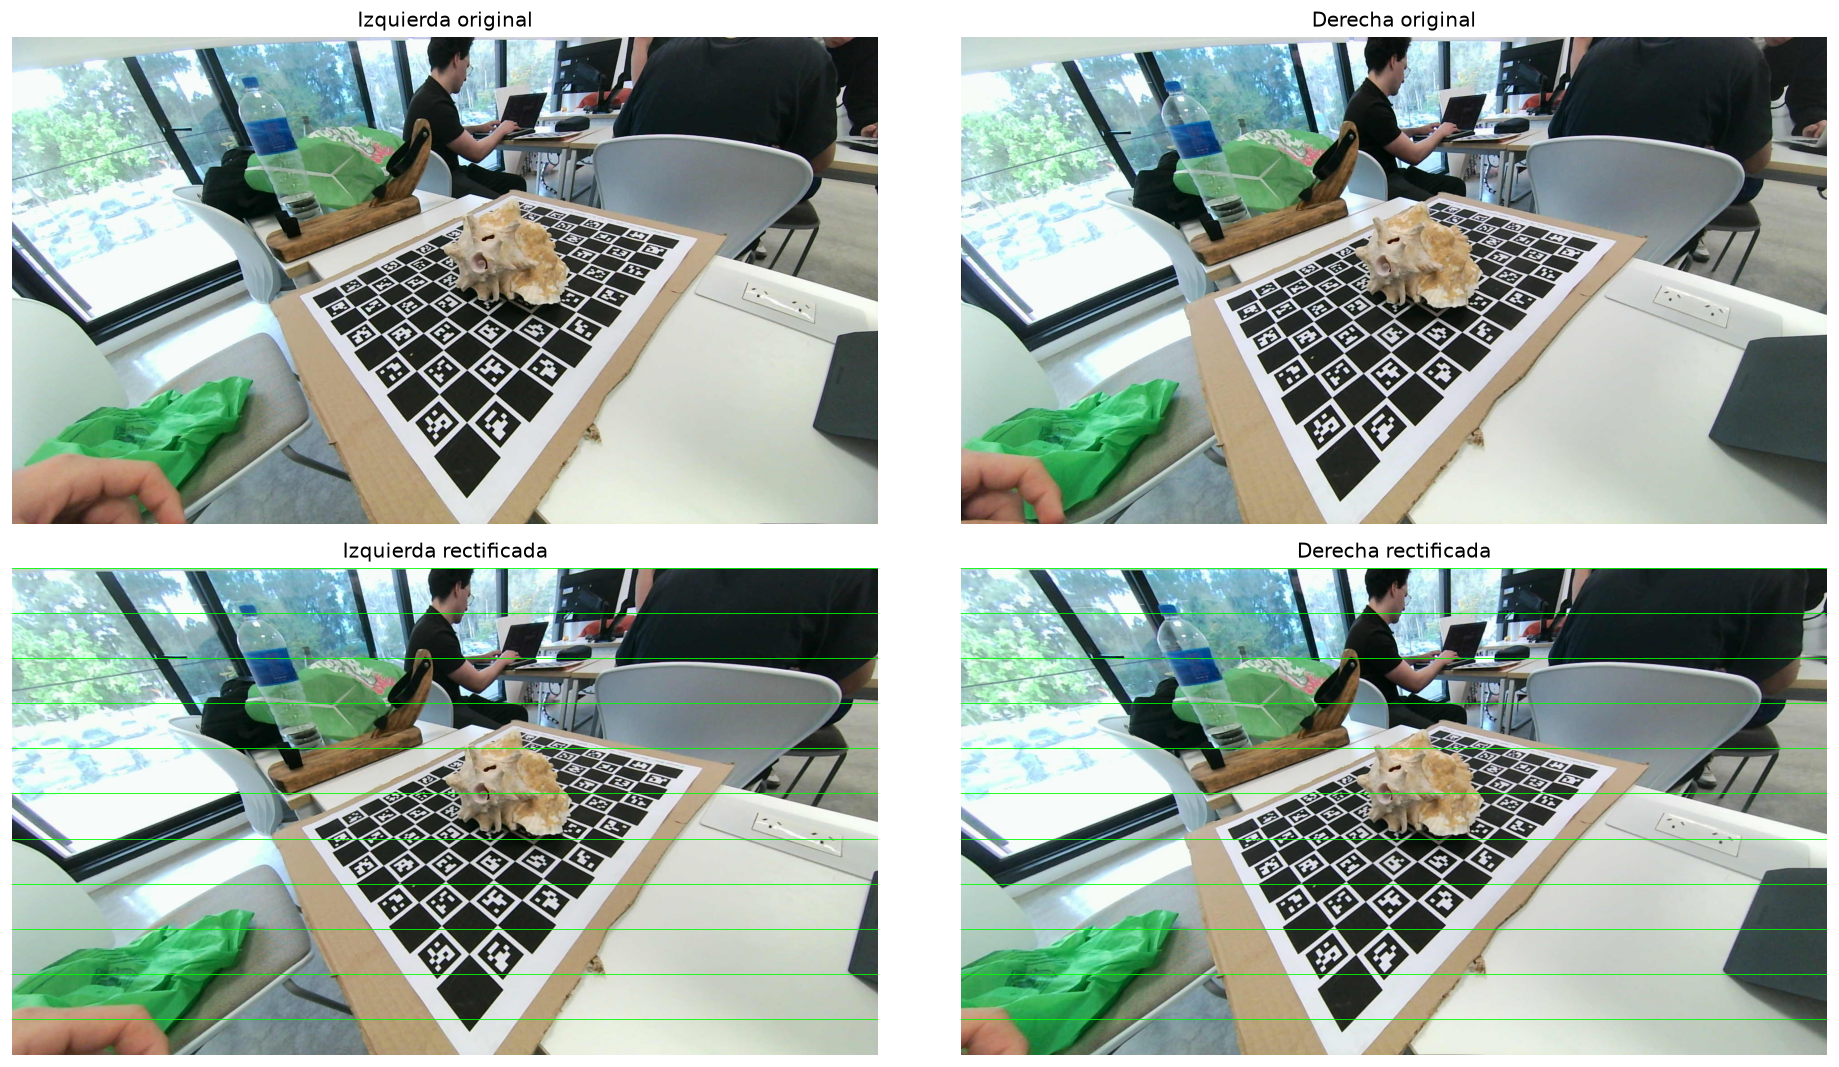
\includegraphics[width=0.78\linewidth]{rectificacion.png}
\caption{Par original (arriba) y rectificado (abajo, con líneas horizontales cada 100\,px), captura 1.}
\label{fig:rect}
\end{figure}

\subsection{Disparidad, nube local y poses}

\begin{figure}[!htb]
\centering
\begin{subfigure}{0.43\linewidth}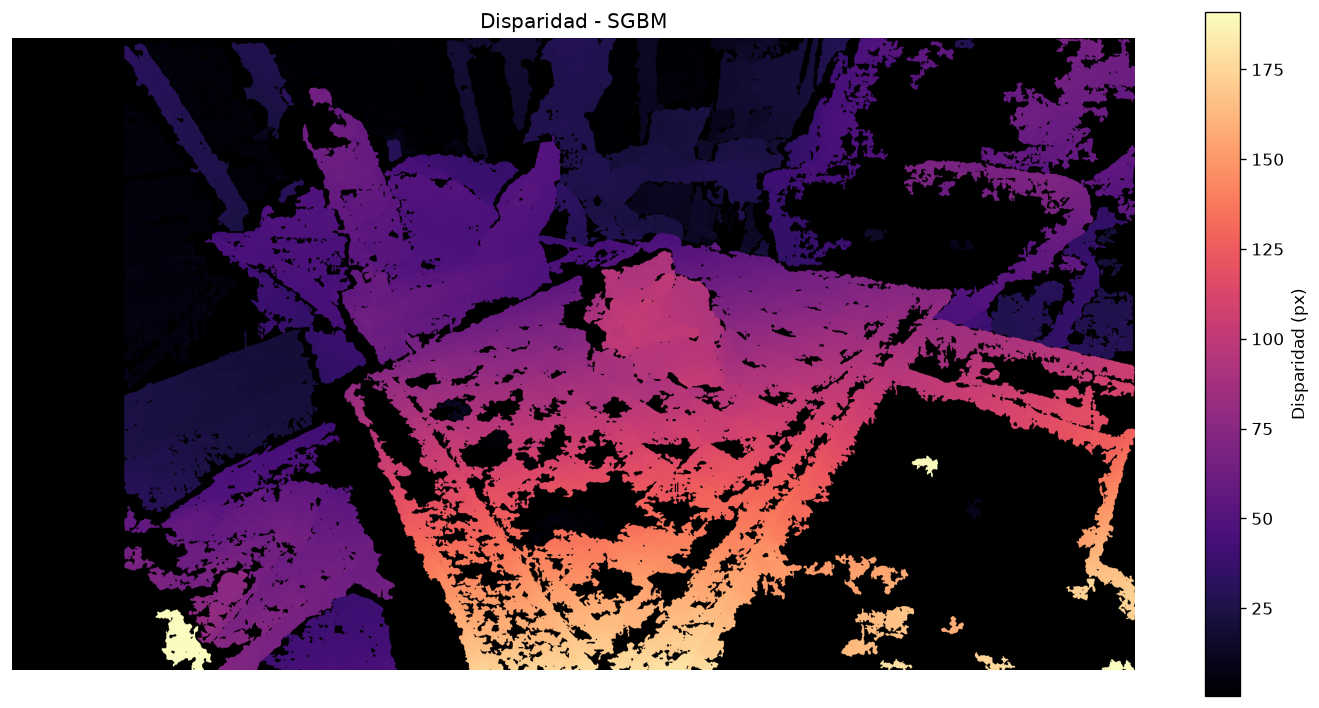
\includegraphics[width=\linewidth]{disparidad.png}\caption{Disparidad SGBM.}\end{subfigure}
\begin{subfigure}{0.28\linewidth}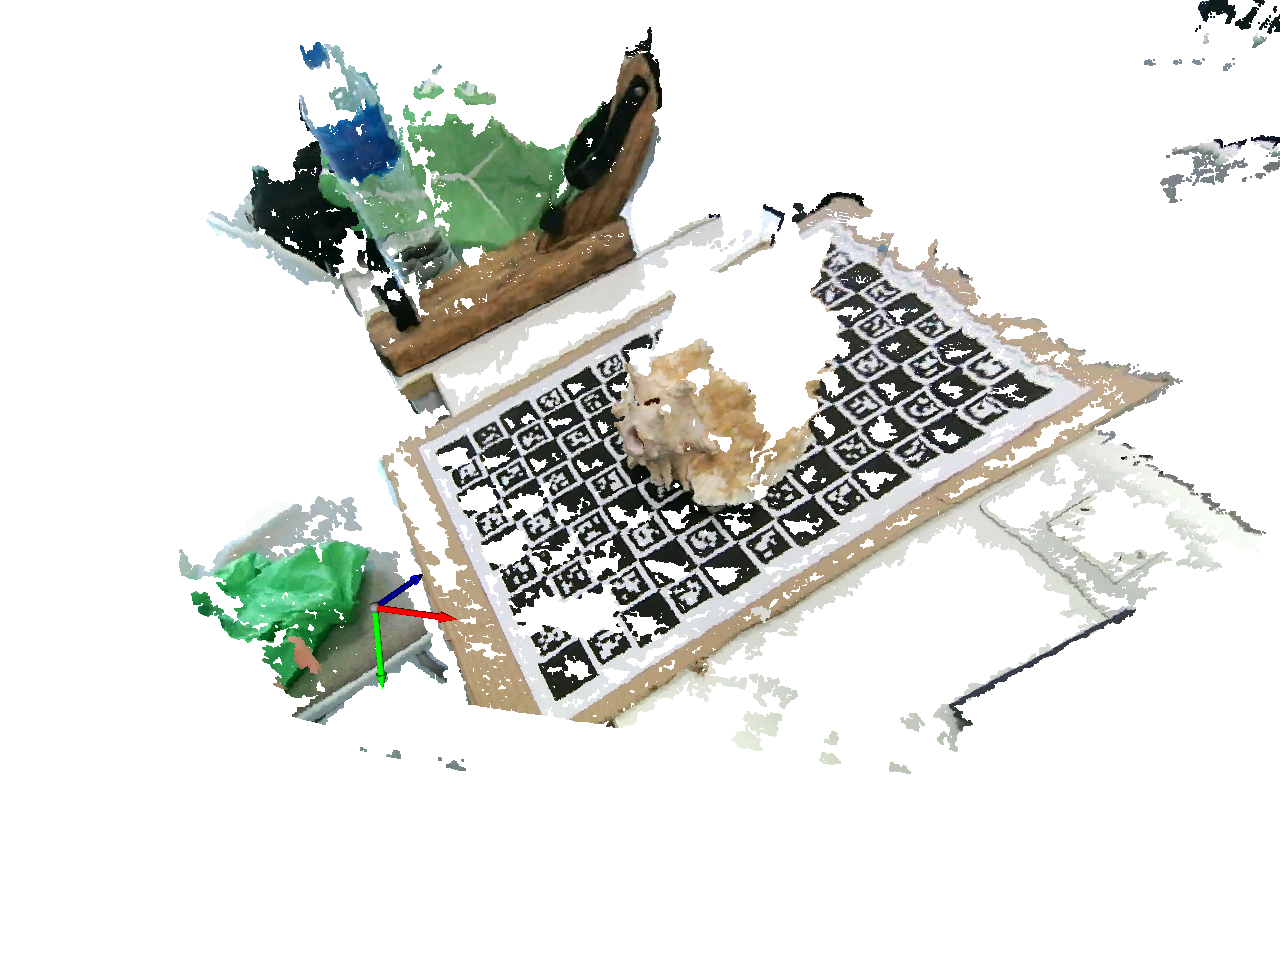
\includegraphics[width=\linewidth,trim=150 250 150 250,clip]{nube_local.png}\caption{Nube local (cámara rectificada).}\end{subfigure}
\begin{subfigure}{0.27\linewidth}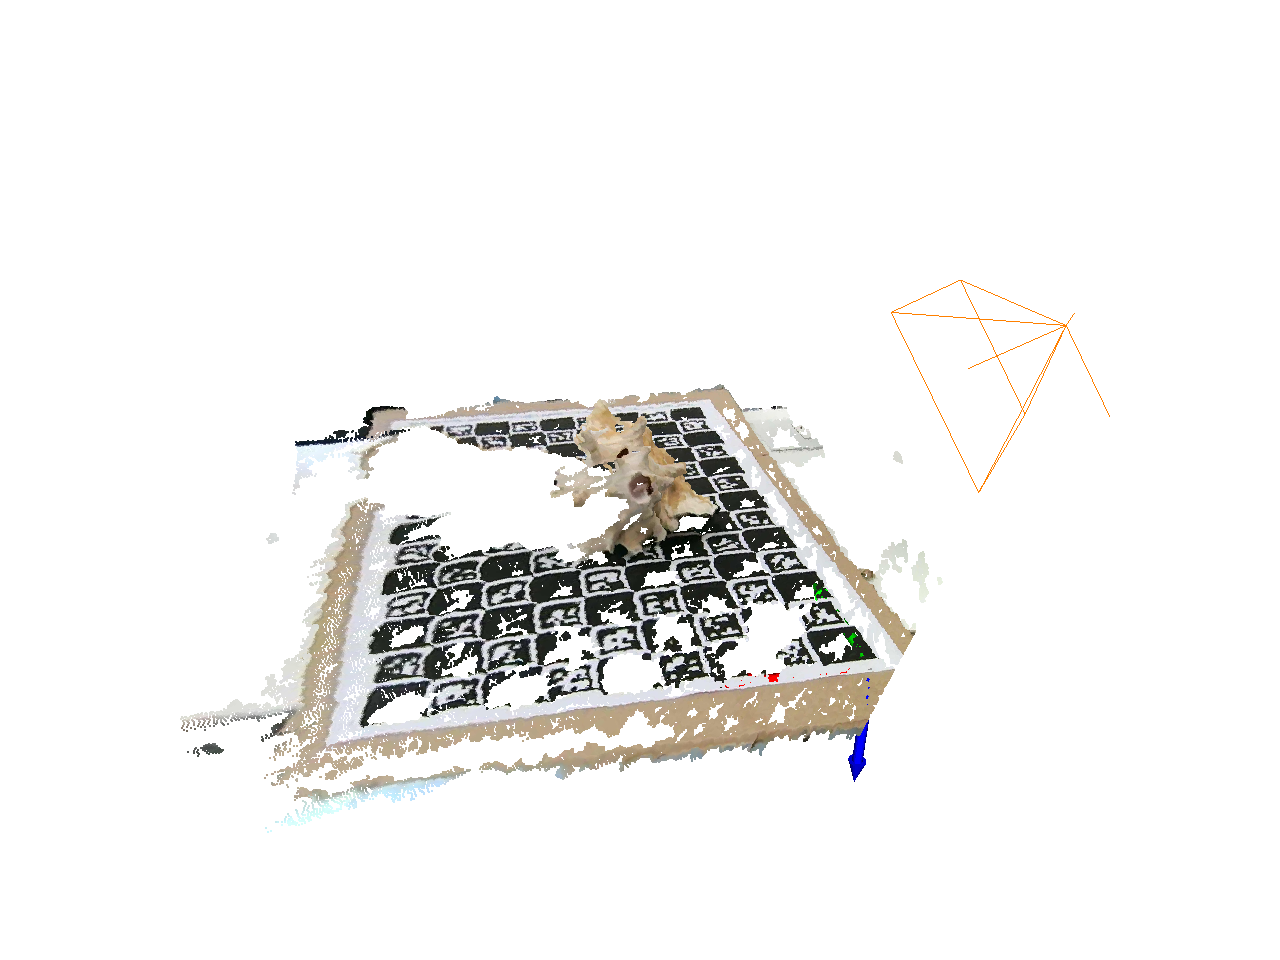
\includegraphics[width=\linewidth,trim=150 200 50 150,clip]{nube_mundo.png}\caption{Nube en el marco del tablero.}\end{subfigure}
\caption{Captura 1. En (c) se ven los ejes del mundo (esquina del ChArUco, $z$ en azul hacia la mesa) y el frustum de la cámara.}
\label{fig:disp}
\end{figure}

La Figura~\ref{fig:disp} muestra un mapa de disparidad representativo: el 67\,\% de los píxeles
tiene disparidad válida (entre 42\,\% y 79\,\% según la captura). El caracol queda en
$d\approx100$--$125$\,px ($Z\approx280$--$350$\,mm). Los huecos se concentran en los cuadros negros
y en la mesa blanca, donde no hay textura, y en las 192 columnas de la izquierda, que no tienen
correspondencia posible. En la parte inferior, la más cercana a la cámara, la disparidad se satura
cerca de 192 px: ahí \texttt{numDisparities} se queda corto, pero esa zona cae fuera del objeto. La
nube local de cada par tiene entre 0.9 y 1.6\,M de puntos.

Se aceptaron 77 de 83 capturas. La 33 se rechazó porque el tablero ocupa el 1.5\,\% de la imagen,
y las 71, 74--76 y 78 porque detectan menos de 8 esquinas (el objeto o el encuadre ocultan el
tablero). El RMS de reproyección de \texttt{solvePnP} es de 1.05\,px en mediana (0.41--2.86\,px). La
Figura~\ref{fig:poses} muestra las poses estimadas: las cámaras rodean el tablero por completo,
a alturas de 35 a 590\,mm y a 100--475\,mm del centro, con los ejes ópticos apuntando hacia el
objeto. Eso coincide con la órbita a mano alzada, de alturas variables, con la que se tomaron
las capturas, y la numeración avanza alrededor del tablero en el orden en que se recorrió.

\begin{figure}[!htb]
\centering
\begin{subfigure}{0.62\linewidth}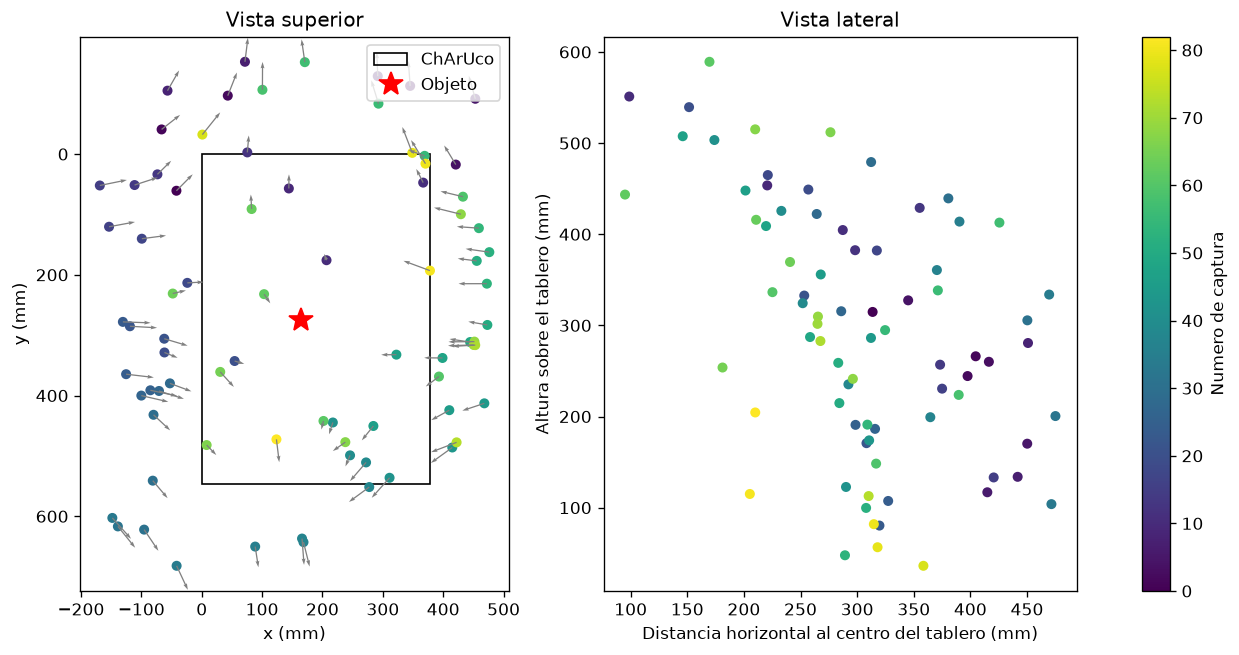
\includegraphics[width=\linewidth]{trayectoria_camaras.png}\end{subfigure}
\begin{subfigure}{0.33\linewidth}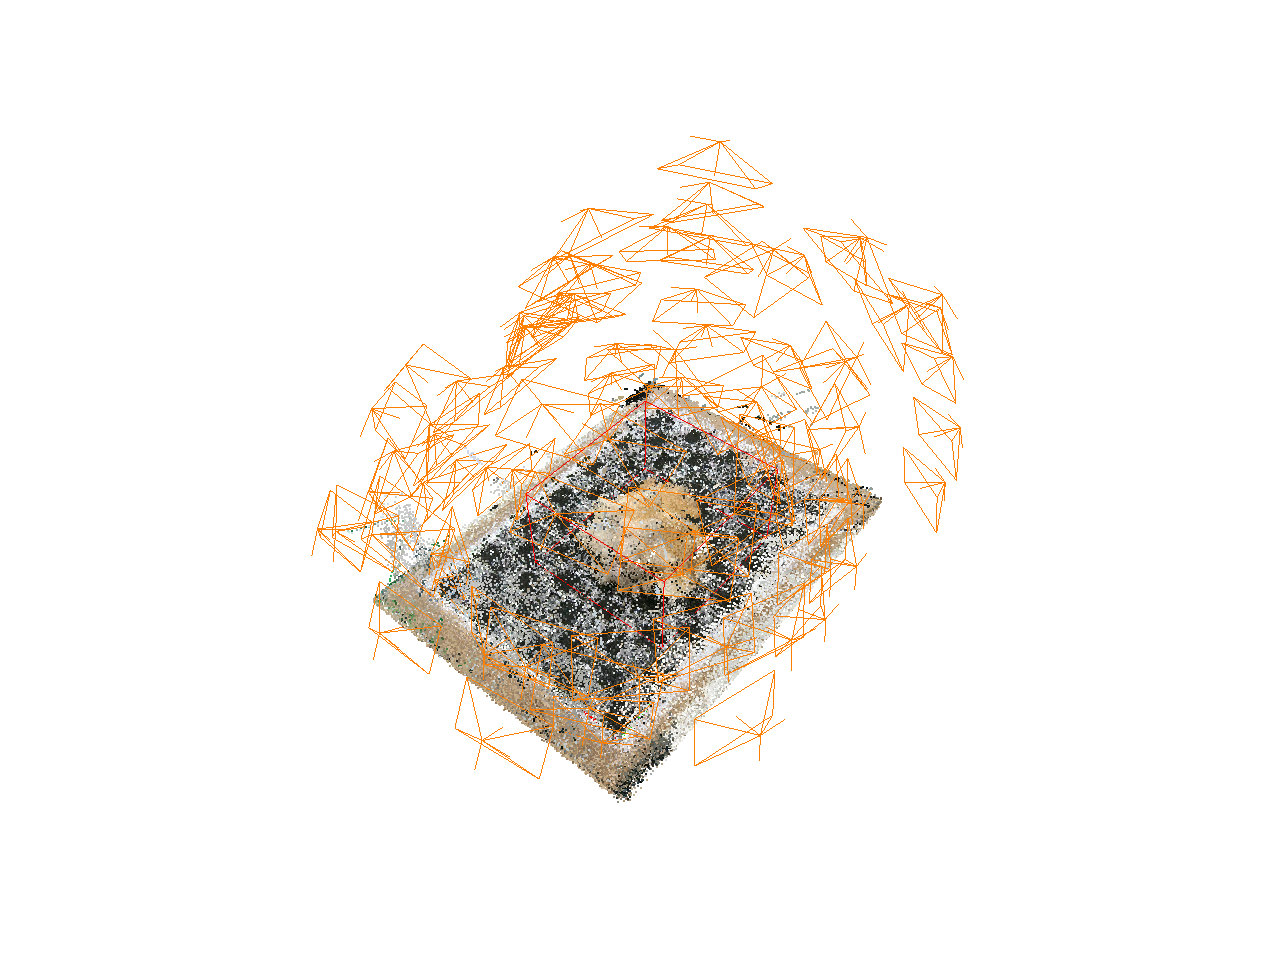
\includegraphics[width=\linewidth,trim=280 100 280 100,clip]{poses_camaras.png}\end{subfigure}
\caption{Poses de las 77 cámaras en el marco del ChArUco. Izquierda: centros (color = número de captura) y dirección del eje óptico. Derecha: frustums sobre la escena fusionada y la caja del objeto (rojo).}
\label{fig:poses}
\end{figure}

\subsection{Fusión y optimización}

La corrección por plano del tablero resultó de $0.55^\circ$ y 3.9\,mm en mediana (máximo de
19.4\,mm). Esto es consistente con el desvío de escala
de $\pm1.6$\,\% entre vistas de la Tabla~\ref{tab:valid}: a 500\,mm, un 2\,\% equivale a 10\,mm. El ICP posterior bajó
el RMSE medio entre cada captura y la referencia de 1.37 a 1.18\,mm (desplazamiento mediano de
4.2\,mm), y aumentó un 41\,\% los puntos que pasan el filtro multivista (de 2.48\,M a 3.50\,M), lo
que indica un mejor empalme.

\begin{table}[!htb]
\centering\small
\begin{tabular}{lrr}
\toprule
Etapa & Puntos & \% del anterior\\
\midrule
Escena completa (77 nubes, sin optimizar) & 104\,748\,216 & --\\
Caja del objeto (\texttt{OrientedBoundingBox}) & 5\,435\,170 & 5.2\,\%\\
ICP + consistencia multivista ($\geq$20 vistas, voxel de 3\,mm) & 3\,495\,281 & 64.3\,\%\\
\texttt{voxel\_down\_sample} (1\,mm) & 259\,442 & 7.4\,\%\\
\texttt{remove\_statistical\_outlier} (30, $2\sigma$) & 247\,529 & 95.4\,\%\\
Cluster DBSCAN principal (\textbf{final}) & \textbf{243\,961} & 98.6\,\%\\
\bottomrule
\end{tabular}
\caption{Puntos sobrevivientes en cada etapa. El \texttt{.ply} final binario (posición, color y normales) pesa 12.4\,MB, mientras que la escena completa ocuparía $\sim$2.8\,GB (posición en \texttt{double} + color).}
\label{tab:stages}
\end{table}

\begin{figure}[!htb]
\centering
\begin{subfigure}{0.24\linewidth}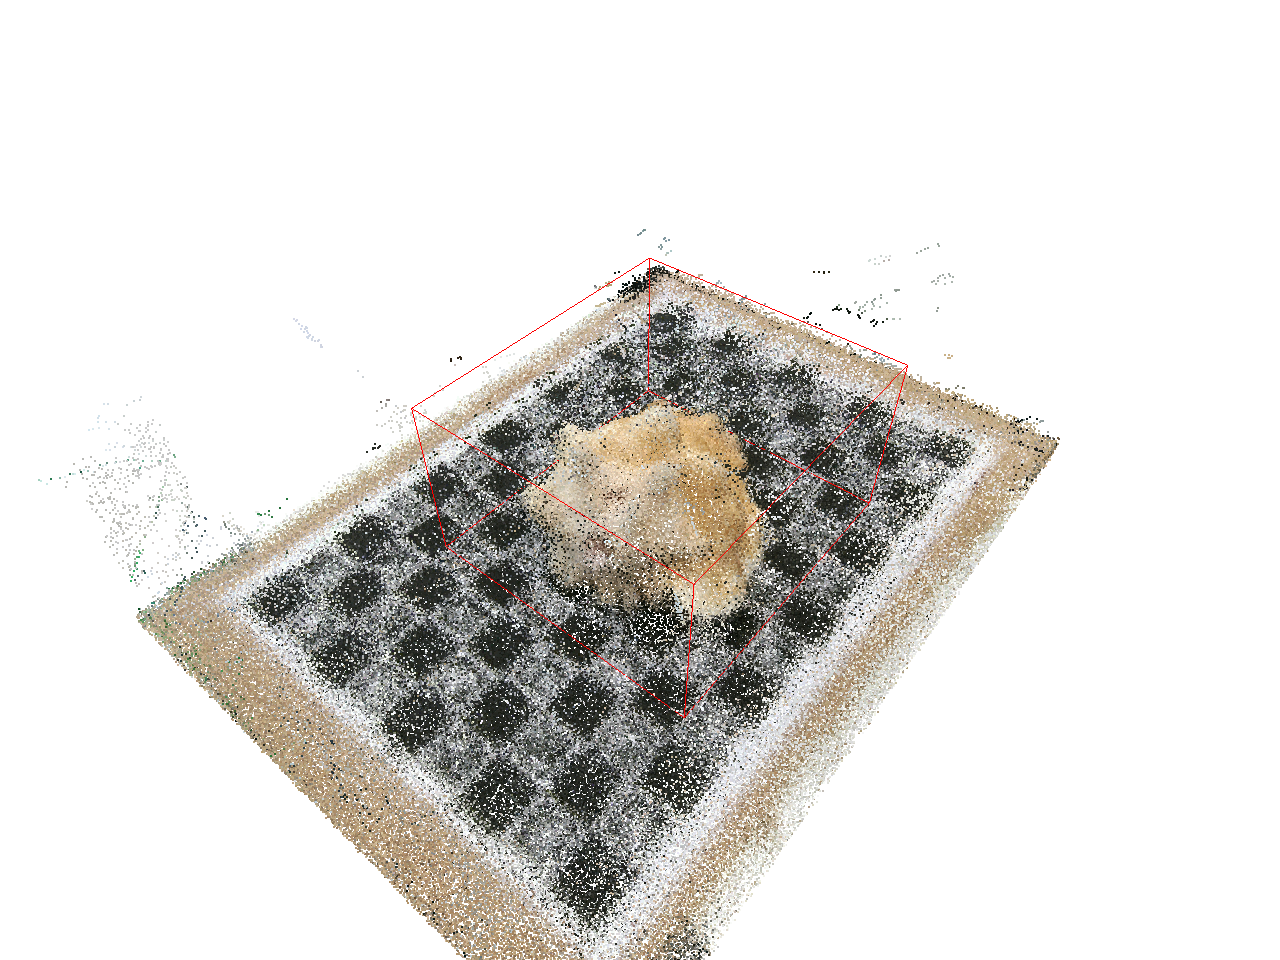
\includegraphics[width=\linewidth,trim=100 100 100 100,clip]{etapa_escena.png}\caption{Escena + caja.}\end{subfigure}
\begin{subfigure}{0.24\linewidth}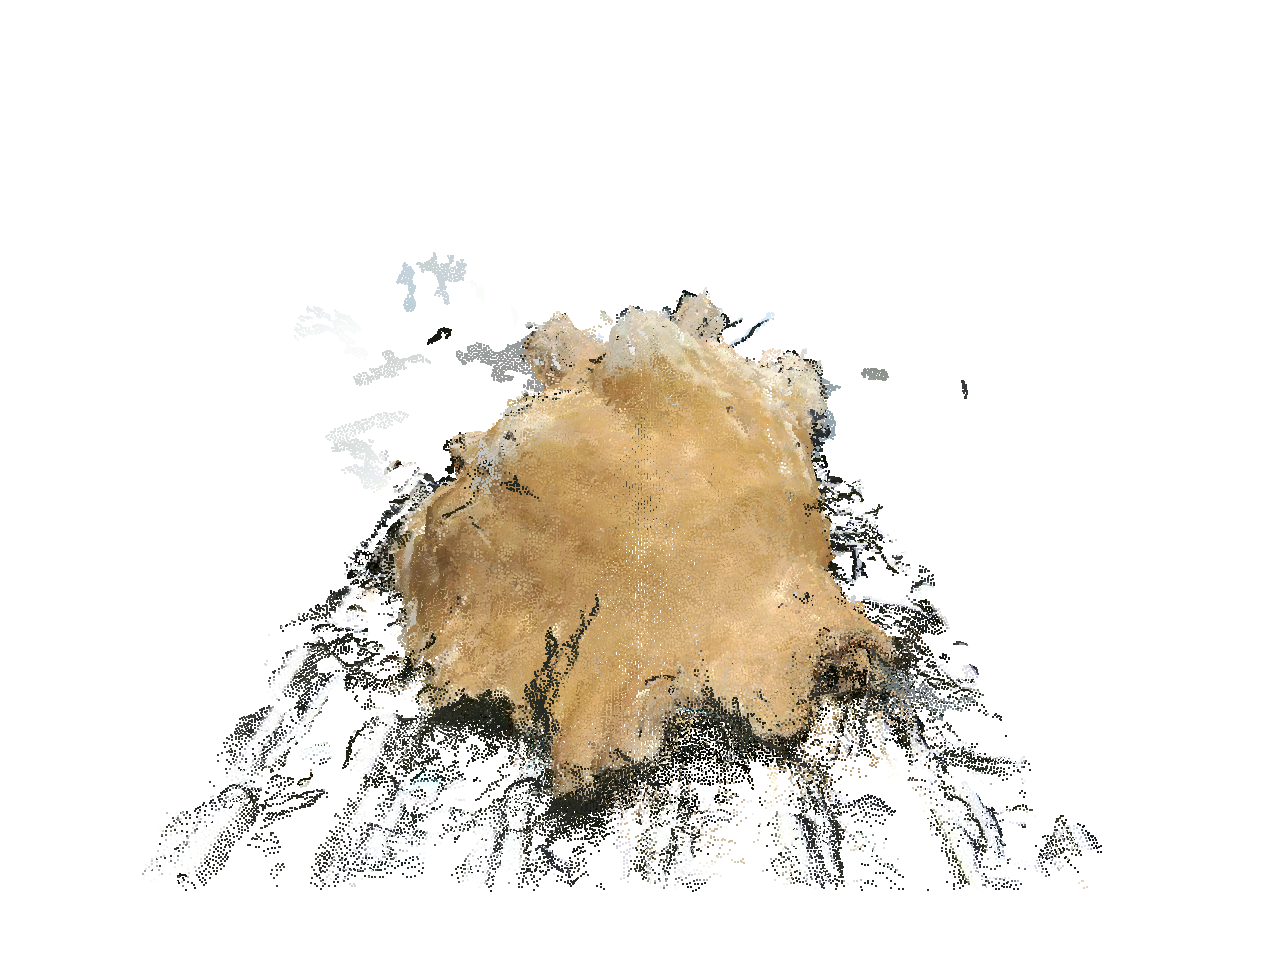
\includegraphics[width=\linewidth,trim=100 150 100 100,clip]{etapa_caja.png}\caption{Recorte con la caja.}\end{subfigure}
\begin{subfigure}{0.24\linewidth}\includegraphics[width=\linewidth,trim=250 200 200 100,clip]{etapa_consistencia_voxel.png}\caption{Multivista + voxel.}\end{subfigure}
\begin{subfigure}{0.24\linewidth}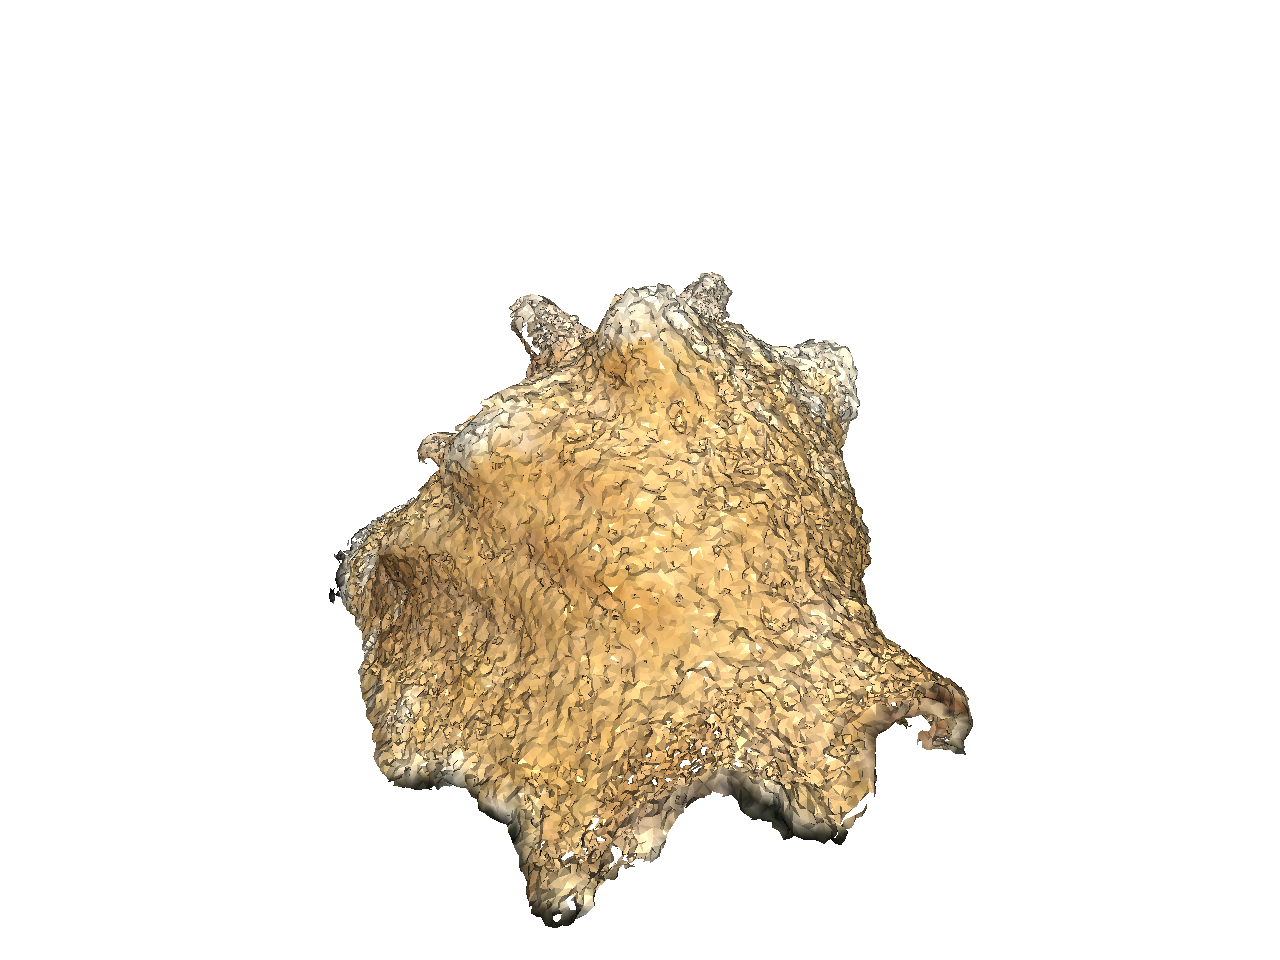
\includegraphics[width=\linewidth,trim=250 200 200 100,clip]{malla_poisson.png}\caption{Malla de Poisson.}\end{subfigure}\\[0.3em]
\begin{subfigure}{0.32\linewidth}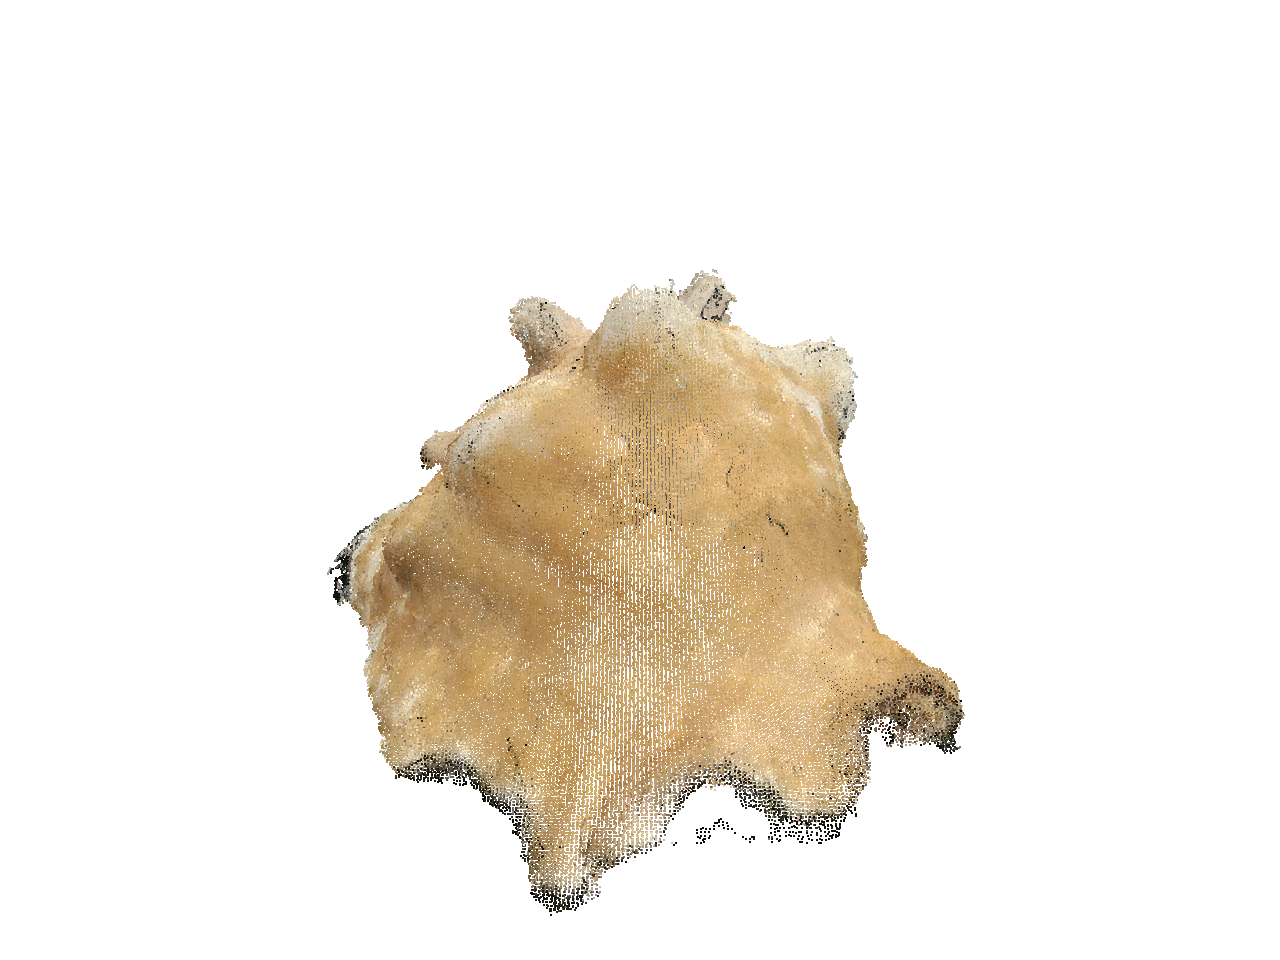
\includegraphics[width=\linewidth,trim=250 200 200 100,clip]{final_frente.png}\end{subfigure}
\begin{subfigure}{0.32\linewidth}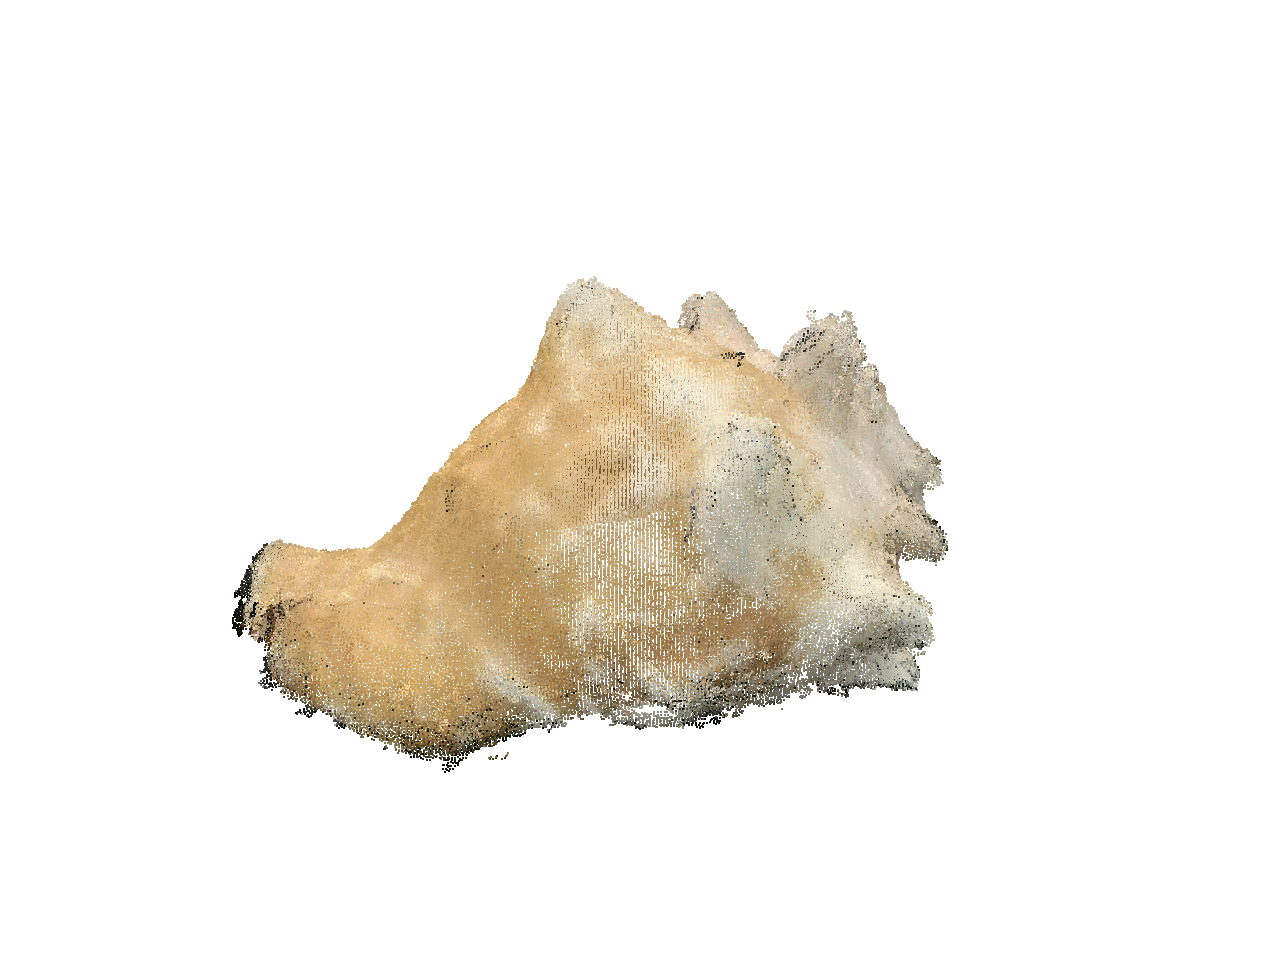
\includegraphics[width=\linewidth,trim=250 200 200 100,clip]{final_lado.png}\end{subfigure}
\begin{subfigure}{0.32\linewidth}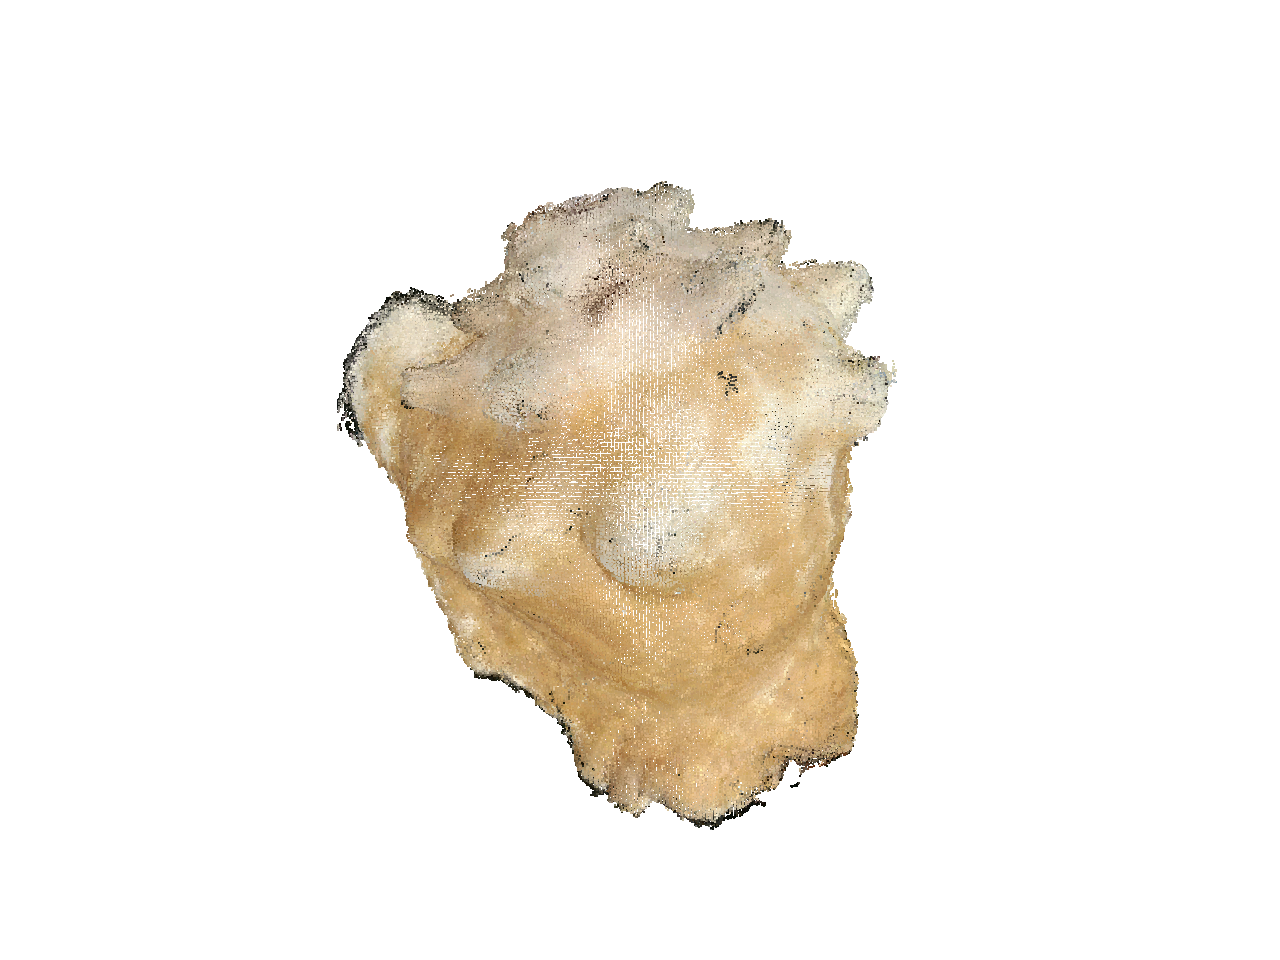
\includegraphics[width=\linewidth,trim=250 150 250 100,clip]{final_arriba.png}\end{subfigure}
\caption{Arriba: etapas de la optimización. Abajo: nube final optimizada desde el frente, de costado y desde arriba.}
\label{fig:stages}
\end{figure}

La Figura~\ref{fig:stages}(b) muestra el principal problema después del recorte: una ``pollera'' de
puntos blancos y negros del tablero que sube por los costados del caracol, además de fragmentos
flotantes. Son \emph{flying pixels}, píxeles en bordes de profundidad a los que SGBM asigna una
disparidad intermedia entre el objeto y el fondo. El filtrado estadístico solo no alcanzaba a
quitarlos, porque son densos localmente. El filtro multivista sí lo logra, porque cada vista
genera la pollera en un lugar distinto (c). El submuestreo a 1\,mm deja la nube en un 7.4\,\% y
conserva las espinas y el labio del caracol.

\subsection{Medición métrica}

\begin{figure}[!htb]
\centering
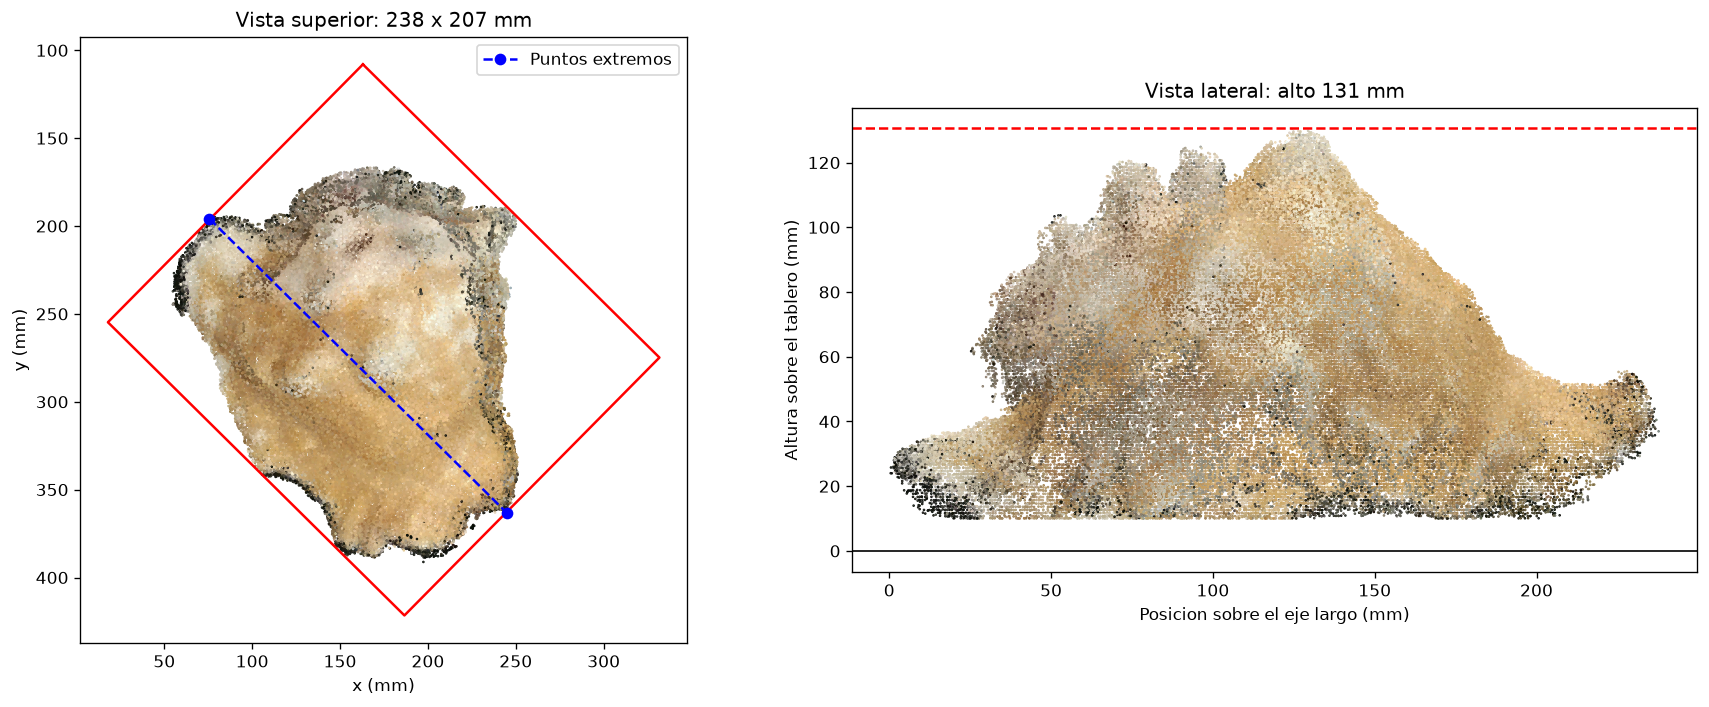
\includegraphics[width=0.85\linewidth]{medicion.png}
\caption{Medición sobre la nube final: rectángulo de área mínima de la proyección sobre el tablero (izquierda) y perfil a lo largo del eje largo, con el plano $z=0$ y el alto (derecha).}
\label{fig:measure}
\end{figure}

\begin{table}[!htb]
\centering\small
\begin{tabular}{lccccc}
\toprule
 & Rectángulo mínimo + plano & OBB mínima Open3D & Rango en 3 corridas & Real (regla) & Error relativo\\
\midrule
Alto  & \textbf{121.8} & 116.2 & 121.7--121.8 & \real{?} & \real{?}\\
Largo & \textbf{219.3} & 221.2 & 216.6--219.3 & \real{?} & \real{?}\\
Ancho & \textbf{202.0} & 209.6 & 201.7--202.2 & \real{?} & \real{?}\\
\bottomrule
\end{tabular}
\caption{Dimensiones estimadas del caracol, en mm.}
\label{tab:measure}
\end{table}

La Tabla~\ref{tab:measure} resume la medición. Usamos como resultado el método que aprovecha el
plano del tablero (Figura~\ref{fig:measure}), porque el alto queda definido respecto de la
superficie de apoyo real. La OBB mínima de Open3D no restringe la orientación y se inclina para
abrazar el objeto, por lo que mezcla alto con ancho (116 vs.\ 122\,mm). Ejecutamos el pipeline
completo tres veces: como el RANSAC de la corrección por plano no es determinista, las medidas
varían en un rango de hasta 2.7\,mm (1.2\,\%), una cota de la repetibilidad del método. El
sesgo medio de escala de la calibración validada es del 0.02\,\%, y el desvío por vista
($\pm1.6$\,\%) se promedia entre las 77 capturas y queda compensado por ICP, así que la escala
no es la fuente dominante: pesan más la definición de los bordes (la base del labio, que toca el
tablero, y la punta de las espinas) y el ruido residual en el contorno.

\subsection{Discusión}

\textbf{Problemas encontrados.} \emph{(1)} Los \emph{flying pixels} de SGBM fueron el principal
obstáculo para tener una nube limpia, y los resolvimos con el filtro de consistencia multivista.
\emph{(2)} Hay una inconsistencia de escala de $\pm$1.6\,\% por vista entre la triangulación y la
pose PnP. La atribuimos a que la profundidad depende de la baseline y de la disparidad, mientras
que la pose depende de $K$ y del tamaño del tablero, y los errores de calibración afectan a cada
una de forma distinta. La compensamos con la corrección por plano y con ICP. \emph{(3)} La
calibración con checkerboard tenía un sesgo de escala del 1.85\,\% en las distancias de captura,
que corregimos con el refinamiento de $(R,\mathbf{t})$. Esto subraya que el RMS de reproyección
por sí solo no garantiza precisión métrica. \emph{(4)} En 6 capturas el tablero no fue detectable.

\textbf{Limitaciones.} El error de profundidad crece como $Z^2$: con $f\!=\!600$\,px y $B\!=\!59$\,mm,
un error de 0.5\,px en la disparidad equivale a $\sim$1.3\,mm a 300\,mm, pero a $\sim$4.3\,mm a
550\,mm. Las vistas lejanas aportan menos precisión. La base del objeto apoyada sobre el tablero
nunca es visible, así que la nube no es cerrada y la malla de Poisson inventa esa cara. Las
zonas sin textura (interior blanco de la abertura) quedan con menos densidad. La caja del objeto
se eligió a mano, a partir de una fusión preliminar.

\textbf{Mejoras posibles.} Usar estéreo con redes neuronales (RAFT-Stereo, CREStereo), que da
disparidades más completas y bordes más nítidos. Ajustar por \emph{bundle adjustment} todas las
poses junto con las esquinas del ChArUco. Fusionar volumétricamente (TSDF), que promedia la
profundidad en lugar de acumular puntos. Capturar más cerca y a distancia constante (por
ejemplo, con un plato giratorio). Calibrar a las mismas distancias de trabajo de la captura.

\end{document}
